\documentclass[10pt]{amsart}
\usepackage[a4paper,margin=23mm]{geometry}
\usepackage{amsmath,amssymb,amsthm,xfrac,hyperref,xspace,graphicx}
\usepackage[english]{babel}
\usepackage[scr=rsfs,cal=euler]{mathalfa}
\newcommand{\resp}{resp.}
\newcommand{\cf}{cf.}
\newcommand{\ie}{i.e.}
\newcommand{\eg}{e.g.}
\newcommand{\loccit}{loc.\ cit.}
\newcommand{\skpt}{\par\smallskip\noindent}
\let\Subsection\subsection
\let\Subsubsection\subsubsection
\emergencystretch=3em
\pagestyle{plain}
\usepackage{enumitem}
\providecommand{\1}{}



%\usepackage{graphicx}
%\usepackage{amsfonts,amssymb,amsmath,amsthm,mathrsfs, verbatim,enumitem,hyperref, mathtools}
\usepackage{mathrsfs}
\usepackage{tikz}
\usetikzlibrary{positioning}
\usetikzlibrary{arrows}
%\usepackage{comment}
%\excludecomment{proof}
%\usetikzlibrary{cd,shapes}
%\usepackage{caption}
%\usepackage{subcaption}
%\usepackage{color}


\DeclareMathOperator{\tors}{tors}
\DeclareMathOperator{\supp}{supp}
\DeclareMathOperator{\image}{Im}
\DeclareMathOperator{\torf}{torf}
\DeclareMathOperator{\op}{op}
\DeclareMathOperator{\add}{add}
\DeclareMathOperator{\Hom}{Hom}
\DeclareMathOperator{\End}{End}
\DeclareMathOperator{\ME}{ME}%For minimal extending
\DeclareMathOperator{\ind}{ind}
\DeclareMathOperator{\cov}{cov}
\DeclareMathOperator{\inv}{inv}
\DeclareMathOperator{\module}{mod}


\usepackage[all]{xy}
\newcommand{\kk}{k}
\newcommand{\suppo}{\supp^{\circ}}

%property names
\newcommand{\calE}{\mathcal{E}}
\newcommand{\calF}{\mathcal{F}}
\newcommand{\calG}{\mathcal{G}}
\newcommand{\calI}{\mathcal{I}}
\newcommand{\calS}{\mathcal{S}}
\newcommand{\calT}{\mathcal{T}}
\newcommand{\calY}{\mathcal{Y}}
\newcommand{\GG}{\mathcal{G}}
\newcommand{\FF}{\mathcal{F}}
\newcommand{\onto}{\twoheadrightarrow}

%Algebra
\newcommand{\filt}{\mathscr{F}\Mk ilt}
\newcommand{\covers}{{\,\,\,\cdot\!\!\!\! >\,\,}}
\newcommand{\covered}{{\,\,<\!\!\!\!\cdot\,\,\,}}
\newcommand{\covdown}{\cov_{\downarrow}}
\newcommand{\covup}{\cov^{\uparrow}}
\newcommand{\join}{\vee}
\renewcommand{\Join}{\bigvee}
\newcommand{\Meet}{\bigwedge}
\newcommand{\strictrefines}{{\,{\ll}\,}}
\newcommand{\refines}{\underline{\,{\ll}\,}}
\newcommand{\tran}{\operatorname{tran}}
\newcommand{\Gen}{\operatorname{Gen}}
\newcommand{\ftors}{\operatorname{f-tors}}
\renewcommand{\1}{\hat{1}}
\newcommand{\0}{\hat{0}}
\newcommand{\newword}[1]{\emph{#1}}

%\numberwithin{equation}{section}

%%%%%%%%%%%%%%%%%%%%%%%%%%%%%%%%%%%%%
\newcommand*{\mk}{\mkern -1mu}
\newcommand*{\Mk}{\mkern -2mu}
\newcommand*{\mK}{\mkern 1mu}
\newcommand*{\MK}{\mkern 2mu}

\hypersetup{urlcolor=purple, linkcolor=blue, citecolor=red}


\newcommand*{\romanenumi}{\renewcommand*{\theenumi}{\roman{enumi}}}
\newcommand*{\Romanenumi}{\renewcommand*{\theenumi}{\Roman{enumi}}}
\newcommand*{\alphenumi}{\renewcommand*{\theenumi}{\alph{enumi}}}
\newcommand*{\Alphenumi}{\renewcommand*{\theenumi}{\Alph{enumi}}}
%%%%%%%%%%%%%%%%%%%%%%%%%%%%%%%%%%


%%%%%%%%%%%%%%%%%%%%%%%%%%%%%%%%%%%%%%%%%%%
\newtheorem{theorem}{Theorem}[section]
\newtheorem{proposition}[theorem]{Proposition}
\newtheorem{lemma}[theorem]{Lemma}
\newtheorem{corollary}[theorem]{Corollary}
\theoremstyle{definition}
\newtheorem{definition}[theorem]{Definition}
\newtheorem{example}[theorem]{Example}
\newtheorem{remark}[theorem]{Remark}
\begin{document}
\title{Canonical join faces of finite-dimensional algebra torsion lattices are precisely finite Hom-orthogonal brick collections}
\author{Emily Barnard \and Andrew Carroll \and Shijie Zhu}
\maketitle
\section{Torsion classes, minimal extensions and bricks}
Let $\Lambda$ be a
finite-dimensional associative algebra over a field~$k$, and write
$\tors \Lambda$ for the set of torsion classes of finitely generated
modules over $\Lambda$, partially ordered by containment.
The poset $\tors \Lambda$ is a complete lattice in which the \newword{meet} (or greatest lower bound) $\Meet \{\calT, \calT'\}$ coincides with the intersection $\calT \cap \calT'$, and the \newword{join} (or smallest upper bound) $\Join \{\calT, \calT'\}$ coincides with the iterative extension closure of the union $\calT\cup \calT'$.
In this paper, we study the cover relations $\calT'\covers \calT$ in $\tors \Lambda$.
Recall that a torsion class $\calT'$ \newword{covers} $\calT$ if $\calT\subsetneq \calT'$ and for each $\calY\in \tors\Lambda$, if $\calT\subsetneq \calY \subseteq \calT'$ then $\calY= \calT'$.
\begin{definition}\label{def:min-ext-module}
A module $M$ is a \newword{minimal extending module for $\calT$} if it satisfies the following three properties:
\begin{enumerate}[label={(P\arabic*)}]
 \item Every proper factor of \label{propertyone}
 $M$ is in $\calT$;
 \item If $0\rightarrow M\rightarrow X
 \rightarrow T\rightarrow 0$ is a non-split exact sequence with
 $T\in \calT$, then $X\in \calT$; \label{propertytwo}
 \item $\Hom(\calT, M)=0$. \label{propertythree}
 \end{enumerate}
\end{definition}
The following remarks will be useful. 
Assuming Property~\ref{propertyone}, Property
\ref{propertythree} is equivalent to the fact that $M\notin \calT$. 
Observe that if there is a non-trivial homomorphism from a module in
$\calT$ to $M$, then both the image and cokernel are in $\calT$, and
$M$ is an extension of the cokernel by the image.
Thus, any minimal extending module is indecomposable. 
Indeed, direct summands are proper factors, and torsion classes are closed under direct sums. 

In the statement of the following theorem, and throughout the paper we have the following notation:
We write $[M]$ for the isoclass of the module $M$; $\ME(\calT$) for the set of isoclasses~$[M]$ such that $M$ is a minimal extending module for $\calT$; and $\filt(\calT \cup \{M\})$ for the iterative extension closure of $\calT \cup \{M\}$.

\begin{theorem}\label{main: covers}
Let $\calT$ be a torsion class over $\Lambda$.
Then the map $$\eta_\calT: [M]\mapsto \filt(\calT\cup \{M\})$$ is a bijection from the set $\ME(\calT)$ to the set of $\calT' \in \tors \Lambda$ such that $\calT \covered \calT'$.
\end{theorem}

Recall that a module $M$ is called a \newword{brick} if the
endomorphism ring of $M$ is a division ring. (That is, the non-trivial
endomorphisms are invertible.)

\begin{theorem}\label{main: cor schur}
Let $\Lambda$ be a finite-dimensional associative algebra and $M\in\module\Lambda$.
Then $M$ is a minimal extending module for some torsion class if and
only if $M$ is a brick.
\end{theorem}
(In the statement below $\Gen(M)$ is the closure of $M$ under taking factors and direct sums.)

\begin{theorem}\label{schur modules to join-irreducibles}
Suppose that $M$ is an indecomposable $\Lambda$ module.
Then the map $\zeta:[M]\mapsto \filt(\Gen(M))$ is a bijection from the
set of isoclasses of bricks over $\Lambda$ to the set of of completely join-irreducible elements in $\tors \Lambda$.
\end{theorem}
Our second application characterizes the collections of subsets $A$ of \emph{completely} join-irreducible elements that belong to $\Gamma(\tors \Lambda)$.
For the second statement of the theorem below, recall that $\tors \Lambda$ is finite if and only if $\Lambda$ is $\tau$-rigid finite (and in this case $\tors \Lambda$ is equal to the lattice of functorially finite torsion classes $\ftors \Lambda$).
See~\cite{IRTT} and Remark~\ref{finite case}.
\setcounter{theorem}{7}
\begin{theorem}\label{main: cjr}
Suppose that $\calE$ is a collection of bricks over $\Lambda$.
Then the set $\{\filt(\Gen M):\, M\in \calE\}$ is a face of $\Gamma(\tors \Lambda)$ if and only if each pair $M$ and $M'$ satisfies the compatibility condition known as \newword{hom-orthogonality}:
\[
\dim \Hom_{\Lambda}(M, M') = \dim \Hom_{\Lambda}(M', M) =0.
\]
In particular, if $\Lambda$ is $\tau$-rigid finite then $\Gamma(\tors \Lambda)$ is isomorphic to the complex of hom-orthogonal $\Lambda$ brick modules.
\end{theorem}
\section{Cover classification core}
\subsection{Preliminaries}\label{sec: background torsion classes}
Throughout, we take $\Lambda$ to be a finite-dimensional associative
algebra over a field $k$, and we write $\module\Lambda$ for the category of finite-dimensional (left) modules over $\Lambda$.
For $\calT$ a class of modules over $\Lambda$ (which we assume to be closed
under isomorphism), we write $\ind \calT$ for the set of indecomposable modules $M\in \calT$ and $[\ind\, \calT]$ for the set of isoclasses $[M]$ such that $M\in \ind \calT$.

A \newword{torsion class} $\calT$ is a class of modules that is closed under factors, isomorphisms, and extensions.
Dually, a class of modules $\calF$ is a \newword{torsion-free class} if it is closed under submodules, isomorphisms, and extensions.
As in the introduction, $\tors \Lambda$ denotes the lattice of torsion classes over $\Lambda$, in which $\calT\le \calT'$ if and only if~$\calT\subseteq \calT'$.
We write $\torf \Lambda$ for the lattice of torsion-free classes also ordered by containment.

At times it will be useful to translate a result or a proof from the language of torsion classes to the language of torsion-free classes.
To do this, we make use of the following standard dualities.
Given a torsion class $\calT$, denote by $\calT^\perp$ the set of modules $X\in
\module \Lambda$ such that $\Hom_\Lambda(\calT, X) = 0$.
The map $(-)^\perp: \tors \Lambda \rightarrow \torf \Lambda$ is a poset
anti-isomorphim with inverse given by $$\calF \mapsto ^\perp
\calF:=\{X\in \module \Lambda:\, \Hom_\Lambda(X, \calF)=0\}.$$
The duality functor $D=\Hom_k(-,k): \module \Lambda \rightarrow \module \Lambda^{\op}$ also furnishes a poset anti-isomorphism from $\tors
\Lambda$ to $\torf \Lambda^{\op}$ with inverse given by the same duality.
(Recall that $\Lambda^{\op}$ denotes the opposite algebra of
$\Lambda$. For details, see~\cite{IRTT} or~\cite{S}.)

Let $\calS$ be a set of indecomposable modules in $\module\Lambda$.
An \newword{$\calS$-filtration (of length $l$)} of a module $M$ in $\module\Lambda$ is a sequence of
submodules \[M=M_l \supsetneq M_{l-1} \supsetneq \cdots
 \supsetneq M_1
\supsetneq M_0=0\] such that $M_i/M_{i-1}$ is isomorphic to a module in $\calS$ for each $i=1,\dotsc, l$.
We write $\filt^{(l)}(\calS)$ for the class of modules $M$ that admit an $\calS$-filtration of length at most~$l$ and $\filt(\calS)$ for the class of all modules in $\module \Lambda$ that admit an $\calS$-filtration, \ie
$\filt(\calS)=\bigcup_{l\geq 0} \filt^{(l)}(\calS)$.
When $\calS$ is not a class of indecomposable modules (but rather an additive full subcategory, for instance) we abuse the notation and write $\filt(\calS)$ instead of $\filt(\ind \calS)$.
We close this subsection with two lemmas.
%Both statements are valid for abelian categories, but we will state them here in the context of modules.
%The notion $\filt(\calS)$ can be generalized for an additive full subcategory $\mathcal C$ in $\module\Lambda$ which is closed under summands by defining $\filt(\calC):=\filt(\ind\calC)$, where $\ind\calC$ denotes a set of representatives isoclasses of all indecomposable modules in $\calC$.

\begin{lemma}\label{lem-ext-closure}
 Let $\calS$ be a class of indecomposable modules in $\module\Lambda$. The class $\filt(\calS)$ is closed under extensions.
\end{lemma}

\begin{proof} Suppose there is an exact sequence
 \[
 0\rightarrow N\rightarrow M\stackrel{\pi}\rightarrow N^\prime\rightarrow 0
 \]
 with $N\in \filt^{(l)}(\calS)$ and $N^\prime\in\filt^{(l^\prime)}(\calS)$.

 Let
 $N=N_l \supsetneq N_{l-1} \supsetneq \dotsc
 \supsetneq N_0 = 0$ and $N^\prime=N^\prime_{l^\prime} \supsetneq N^\prime_{l^\prime-1} \supsetneq \dotsc
 \supsetneq N^\prime_0 = 0$ be an $\calS$-filtration of $N$ and
 $N^\prime$ respectively. Take $M_{i}$ to be the pull back following, for $0\leq
 i\leq l^\prime$:
\[
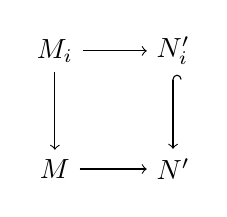
\begin{tikzpicture}[scale=0.75]
 \node (A) at (0,0) {$M_i$}; 
 \node(B) at (2,0) {$N_i'$};
 \node (C) at (0,-2) {$M$}; 
 \node (D) at (2,-2) {$N'$};
 \draw[->] (A.east)--(B.west);
 \draw[->] (A.south)--(C.north);
 \draw[->] (C.east)--(D.west);
 \draw[right hook->] (B.south)--(D.north);
\end{tikzpicture}
\]
Then $M=M_{l^\prime} \supsetneq M_{l^\prime-1}\supsetneq \cdots
 M_0=N=N_l \supsetneq N_{l-1} \supsetneq \cdots
 \supsetneq N_0 = 0$ is an $\calS$-filtration of $M$.
\end{proof}


\begin{lemma}\label{lem-epi-closure}
Suppose that $\calS$ is a class of indecomposable modules that is
closed under taking indecomposable summands of factors.
Then $\filt(\calS)$ is closed under factors.
Dually, if $\calS$ is closed under taking indecomposable summands of submodules, then $\filt(\calS)$ is closed under submodules.
\end{lemma}
\begin{proof}
 Suppose that $N\in \filt^{(l)}(\calS)$ and $\phi: N\rightarrow U$ is an epimorphism.
We assume, without loss of generality, that $U$ is indecomposable and proceed by induction on $l$.
If $l=1$, then $N\in \calS$.
% so $U$ is an indecomposable factor of $N$.
Since $\calS$ is closed under epimorphisms, we have $U\in \calS$.
Now suppose that all factors of modules in $\filt^{(l^\prime)}(\calS)$
are in $\filt(\calS)$ for $l'<l$.
Since $N\in \filt^{(l)}(\calS)$, it admits an $\calS$-filtration $N=N_l\supsetneq N_{l-1} \supsetneq \cdots
\supsetneq N_0=0$ with $N_i/N_{i-1}$ isomorphic to an object in
$\calS$. Consider the submodule $\phi(N_{l-1})$ of $U$, and notice that $\phi(N_{l-1})$ is a factor of $N_{l-1}\in \filt^{(l-1)}(\calS)$.
Therefore, by induction, $\phi(N_{l-1})$ has an $\calS$-filtration.
% \[ \phi(N_{l-1})=U_t\supsetneq U_{t-1} \supsetneq \dotsc \supsetneq U_0 = 0.\]
Further, $U/\phi(N_{l-1})$ is a factor of $N_{l}/N_{l-1}\in\calS$.
Therefore $U/\phi(N_{l-1})$ belongs to $\calS$.
We have the following short exact sequence:
 \[
 0\rightarrow \phi(N_{l-1})\rightarrow U\stackrel{\pi}\rightarrow U/\phi(N_{l-1})\rightarrow 0.
 \]
Lemma~\ref{lem-ext-closure} then implies that $U$ is in $\filt(\calS)$, as desired.
%We prove the dual statement similarly by induction.
%Suppose that $U$ is a submodule of $N$.
%By induction, $U\cap N_{l-1}$ is a member of $\filt(\calS)$, and also $U/(U\cap N_{l-1})$ is a submodule of $N_l/N_{l-1}$.
%Since $\calS$ is closed under submodules and $N_{l}/N_{l-1}$ is a member of $\calS$, we have $U/(U\cap N_{l-1})$ is a member of $\calS$.
%We have the short exact sequence:
%\[ 0 \rightarrow U\cap N_{l-1} \rightarrow U \rightarrow U/(N_{l-1}\cap U) \rightarrow 0.\]
%As above, we conclude that $U\in \filt(\calS)$.
\end{proof}

\subsection{Minimal extending modules}\label{proof sec}
In this subsection, we prove Theorem~\ref{main: covers}.
We begin by showing that $\eta_\calT: [M]\mapsto \filt(\calT \cup \{M\})$ is well-defined.
The first statement in the next lemma confirms that $\filt(\calT \cup \{M\})$ is indeed a torsion class.
Because it follows immediately, we also dispense with the forward direction of Theorem~\ref{main: cor schur}.
\begin{lemma}\label{lem: torsion and schur}
Suppose that $\calT\in \tors \Lambda$ and $M$ is an indecomposable $\Lambda$ module that does not belong to $\calT$.
If every proper factor of $M$ lies in $\calT$ then:
\begin{enumerate}
\item $\filt(\calT \cup \{M\})$ is a torsion class and
\item $M$ is a brick over $\Lambda$.
\end{enumerate}
\end{lemma}
\begin{proof}
The first statement follows immediately from Lemma~\ref{lem-epi-closure}.
To prove the second statement, let $f:M\rightarrow M$ be a non-zero morphism, and assume that $f$ is not an isomorphism.
%We need to show that $f$ is an isomorphism.
Consider the exact sequence:
$$
0\rightarrow \image f\rightarrow M\rightarrow M/\image f\rightarrow 0.
$$
Observe that both $\image f$ and $M/\image f$ are proper factors of $M$, and thus belong to $\calT$.
%Otherwise $0\neq\image f\subsetneq M$ is a proper factor of $M$. By assumption, $\image f\in \calT$.
%Since $\image f\neq 0$, $M/\image f$ is a proper factor of $M$. Hence $M/\image f\in\calT$.
Because $\calT$ is closed under extensions, it follows that $M\in\calT$, and that is a contradiction.
Therefore $\End(M)$ only contains automorphisms
and hence $\End(M)$ is a division ring. So $M$ is a brick.
\end{proof}
\begin{lemma}\label{uniqueness}
Let $\calT\in \tors\Lambda$ and $M\not\in \calT$ be indecomposable such that each proper factor of $M$ belongs to $\calT$.
Let $N\in \filt(\calT \cup \{M\})\setminus \calT$ such that each proper factor of $N$ lies in $\calT$.
If $\filt(\calT \cup \{M\})\covers \calT$ then $N\cong M$.
%Suppose that $N\in \filt(\calT \cup \{M\})\setminus \calT$ satisfies each proper factor $N$ lies in $\calT$.
%Then $N$ is isomorphic to $M$.
 
\end{lemma}
\begin{proof}
Write $\calT'$ for $\filt(\calT \cup \{M\})$.
Note that $N$ also satisfies the assumptions of Lemma~\ref{lem:
 torsion and schur}, so $\filt(\calT \cup \{N\})$ is a torsion class
which properly contains $\calT$ (since $N\notin \calT$) and is
contained in $\calT'$.
Hence, $\calT'=\filt(\calT \cup \{N\})$. 
In particular, $N$ admits a $\calT \cup \{M\}$-filtration with at
least one subfactor isomorphic to $M$, so $\dim N \geq \dim M$. 
Symmetrically, $M$ admits a $\calT \cup \{N\}$-filtration with at
least one subfactor isomorphic to $N$.
Therefore, $M\cong N$. 
\end{proof}

\begin{proposition}\label{prop: epis and covers}
Let $\calT\in \tors\Lambda$ and $M\not\in \calT$ be an indecomposable module such that each proper factor of $M$ belongs to $\calT$.
Then $\calT' =\filt(\calT \cup \{M\}) \covers \calT$ if and only if $M$ is a factor of each $N\in \calT'\setminus \calT$.
\end{proposition}
\begin{proof}
First we argue the ``if'' direction.
Suppose that every element in $\calT'\setminus \calT$ admits an epimorphism to $M$.
Let $\calG$ be a torsion class with $\calT \subsetneq \calG \subseteq \calT'$, and pick $N\in \calG\setminus \calT$.
Because $M$ is a factor of $N$, we have $M\in \calG$.
Thus, $\calT'=\filt(\calT \cup \{M\}) \subseteq \calG$, as desired.

Conversely, suppose that $\calT'\covers \calT$, and let $N$ be any module in $\calT'\setminus \calT$.
Among all submodules $N'\subseteq N$ such that $N/N'\in \calT'\setminus \calT$, choose $N'$ maximal.
By Lemma~\ref{uniqueness} $N/N'$ is isomorphic to $M$.
We conclude $M$ is a factor of $N$.
\end{proof}

We use the previous proposition to verify that $\eta_\calT$ (from Theorem~\ref{main: covers}) has the correct codomain.
In the next proposition, $\covup(\calT)$ denotes the set of torsion classes $\calT'$ such that $\calT' \covers \calT$.
\begin{proposition}\label{thm:pseudo-minimal-covers}
Suppose that $\calT\in \tors \Lambda$ and $M$ is an indecomposable $\Lambda$ module.
If $M$ is a minimal extending module for $\calT$, then $\filt(\calT \cup \{M\})\covers \calT$.
That is, the map $\eta_\calT: \ME(\calT) \to \covup(\calT)$ is well-defined.
\end{proposition}
\begin{proof}
Again, denote by $\calT'$ the torsion class $\filt(\calT\cup \{M\})$. 
Properties~\ref{propertyone} and~\ref{propertythree} imply that $M$ satisfies the hypotheses of Proposition~\ref{prop: epis and covers}.
Let $N\in \calT' \setminus \calT$ with $\ind \calT \cup \{M\}$-filtration $N=N_l\supsetneq N_{l-1} \supsetneq \cdots
 \supsetneq N_0=0$. Assume, without loss of generality, that $N$ is indecomposable. 
We argue by induction on $l$ that $M$ is a factor of $N$.
If $l=1$, then $N\cong M$ since $N\notin \calT$.
Suppose that $l>1$, and let $i$ to be the smallest index such that $N_i/N_{i-1} \cong M$ (one must exist since $N\notin
 \calT$).

If $i=1$, then there is a short exact sequence 
\[0 \rightarrow M \rightarrow N \rightarrow N/N_1 \rightarrow 0.\]
\looseness-1
Since $N$ was assumed indecomposable (and $l>1$), the sequence does
not split.
If $N/N_1 \in \calT$, then by Property~\ref{propertytwo}, $N\in
\calT$, a contradiction.
Otherwise, $N/N_1 \not\in \calT$ is in $\filt^{(l-1)}(\calT\cup \{M\})$,
so by induction, $M$ is a factor of $N/N_1$, so it is also a factor of
$N$. 

If $i>1$, consider the short exact sequence 
\[0 \rightarrow N_{i-1} \rightarrow N \rightarrow N/N_{i-1} \rightarrow 0\]
which again is non-split by assumption.
Note that since $N_{i-1}$ has a filtration by modules in $\calT$, $N_{i-1}\in
\calT$. 
If $N/N_{i-1}\in \calT$, then so is $N$, since torsion classes are
closed under extensions. 
Therefore, $N/N_{i-1} \notin \calT$, and it has a
$\calT\cup\{M\}$-filtration of length $l-i+1<l$.
Hence, by induction, $M$ is a factor of $N/N_{i-1}$, and therefore of $N$ as well. 

Hence, $M$ is a factor of $N$ for each module $N$ in
$\calT'$, so $\calT\lessdot \calT'$. 
\end{proof}

Below we construct the inverse map to $\eta_\calT$, completing the proof of Theorem~\ref{main: covers}.
Recall that $[\ind\, \Lambda]$ is the set of isoclasses $[M]$ such that $M\in \ind \Lambda$.
\begin{theorem}\label{thm: eta inverse}
For each $\calT'\covers \calT$ in $\tors\Lambda$, there exists a unique (up to isomorphism) indecomposable module $M$ such that $\calT' = \filt(\calT \cup \{M\})$.
Furthermore, the map $\filt(\calT \cup \{M\}) \mapsto [M]$ is the inverse to $\eta_\calT$.
\end{theorem}
\begin{proof}[Proof of Theorem~\ref{thm: eta inverse} and Theorem~\ref{main: covers}]
Let $N\in \calT' \setminus \calT$.
As in the proof of Proposition~\ref{prop: epis and covers}, among all submodules $N'$ of $N$ such that $N/N'\in \calT'\setminus \calT$, choose $N'$ maximal.
We take $M$ to be the factor~$N/N'$.
(It is immediate that $M$ is indecomposable.)
Because $\calT'\covers \calT$, we conclude that $\calT' = \filt(\calT \cup \{M\})$.
Lemma~\ref{uniqueness} implies that $M$ is unique up to isomorphism.
%The same argument as given in the second paragraph of the proof of Proposition~\ref{prop: epis and covers} shows that $M$ is unique up to isomorphism.

To prove the second statement, it is enough to show that $M$ is a minimal extending module.
It is immediate that $M$ satisfies Property~\ref{propertyone}.
Suppose that $0\to M \stackrel{i}\rightarrow X\stackrel{\pi}\rightarrow T\rightarrow 0$ is a short exact sequence with $T\in \calT$.
If $X\in \calT'\setminus \calT$, then Proposition~\ref{prop: epis and
 covers} implies that there is an epimorphism $q: X\rightarrow
M$. If $q\circ i=0$, then $q$ factors through $\pi$ which implies that
$M$ is a quotient of $T$, contradicting with $M\notin \calT$. If
$q\circ i\neq 0$, then $q\circ i$ is an isomorphism due to the fact
that $M$ is a brick. So the exact sequence splits.
Thus~$M$ satisfies property~\ref{propertytwo}.
%Assume that $Q\in \calT$ is a module with a non-zero morphism $f:Q\rightarrow M$.
%Without loss of generality we can assume $f$ is a monomorphism, otherwise taking $Q=\image f$.
%Then we have the canonical exact sequence\[0\rightarrow Q \rightarrow M \rightarrow M/Q\rightarrow 0\] in which $M/Q$ is a proper factor of $M$, and therefore lies in $\calT$.
%Thus $M\in \calT$ (because $\calT$ is closed under extensions), and that is a contradiction.
%We conclude that 
By construction, $M\not\in\calT$. Thus according to the first remark after Definition~\ref{def:min-ext-module}, $M$ satisfies~\ref{propertythree}.
\end{proof}
The following corollary will be useful as we explore the connection to
the canonical join complex of $\tors \Lambda$ in
Section~\ref{canonical join complex}.
\begin{corollary}\label{hom orthogonality}
Let $\calT_1$ and $\calT_2$ be distinct torsion classes in $\tors \Lambda$, and for each $i\in \{1,2\}$, let $M_i$ be a minimal extending module for $\calT_i$.
If $\filt(\calT_1 \cup \{M_1\}) = \filt(\calT_2 \cup \{M_2\})$ then \[\dim \Hom_{\Lambda}(M_1,M_2) = \dim \Hom_{\Lambda}(M_2,M_1)=0.\]
\end{corollary}
\begin{proof}
Write $\calT'$ for $\filt(\calT_1 \cup \{M_1\}) = \filt(\calT_2 \cup \{M_2\})$.
First, we claim that $M_1$ belongs to $\calT_2$ and $M_2$ belongs to $\calT_1$.
Then the statement follow immediately from Property~\ref{propertythree} of minimal extending modules.
Since $\calT_1$ and $\calT_2$ are distinct and both covered by the same torsion class $\calT'$, it follows that there exists some $N\in \calT_1\setminus \calT_2$.
In particular, $N\in \calT'\setminus \calT_2$.
Proposition~\ref{prop: epis and covers} implies that $N$ surjects onto $M_2$.
Thus, $M_2\in \calT_1$.
By symmetry $M_1\in \calT_2$.
\end{proof}
\subsection{Torsion-free classes and bricks}
We now record the corresponding notions for
torsion-free classes, both for completeness, and for a convenient
proposition relating the upper covers of $\calT$ to the lower
covers of $\calT^\perp$.
(See Proposition~\ref{prop:torsion-free-to-torsion-relation} below.)
Proofs that are essentially equivalent to their counterparts in the
torsion context are suppressed.
We begin by defining the analogue to minimally extending modules.

\begin{definition}
A module $M$ is called a \newword{minimal co-extending module for a torsion-free class $\calF$} if it satisfies the following
three conditions:
\begin{enumerate}[label={(P\arabic*$'$)}]
\item \label{copropertyone} Every proper submodule of $M$ is
 in $\calF$;
\item \label{copropertytwo} if $0\rightarrow F \rightarrow X
 \rightarrow M \rightarrow 0$ is a non-split exact sequence, with
 $F\in \calF$, then $X\in \calF$;
\item\label{copropertythree} $\Hom_\Lambda(M,\calF)=0$.
\end{enumerate}
\end{definition}
In Theorem~\ref{prop:min-ext-module-free} below, the notation $\covup(\calF)$ is the set of torsion-free classes~$\calF'$ such that $\calF' \covers \calF$.
\begin{theorem}\label{prop:min-ext-module-free}
Suppose that $\calF$ is a torsion-free class over $\Lambda$ and $M\not\in \calF$ is an indecomposable $\Lambda$ module.
The following are equivalent:
\begin{enumerate}
\item $M$ is a minimal co-extending module of $\calF$.
\item Each proper submodule of $M$ lies in $\calF$ and $M$ is a submodule for each $N\in \filt(\calF\cup \{M\})\setminus \calF$.
\item $\filt(\calF \cup\{M\}) \covers \calF$.
\end{enumerate}
The map $\zeta: [M]\mapsto \filt(\calF\cup \{M\})$ is a bijection from the set of isoclasses $[M]$ such that $M$ is a minimal co-extending module for $\calF$ to the set $\covup(\calF)$.
\end{theorem}


\begin{proposition}\label{prop:torsion-free-to-torsion-relation}
Suppose that $\calT$ is a torsion class in $\tors \Lambda$ and $M$ is
an indecomposable $\Lambda$ module such that $\filt(\calT \cup \{M\})$
is a torsion class. Then $M$ is a minimal extending module for the torsion class $\calT$ if and only if it is a minimal co-extending module for the torsion-free class $\filt(\calT \cup\{M\})^\perp$.
\end{proposition}

\begin{proof}
We argue the forward implication of the proposition; the reverse implication is similar. 
Let $\calT'$ denote the torsion class $\eta_\calT([M])=\filt(\calT \cup \{M\})$.
Observe that $M\not\in (\calT')^\perp$.
Also, Property~\ref{propertythree} implies that $M$ belongs to $\calT^\perp$.
By Theorem~\ref{prop:min-ext-module-free}, it is enough to show that $M$ satisfies the following:
First, each proper submodule of $M$ belongs to $(\calT')^\perp$; and second, $M$ is a submodule of each $X\in \calT^\perp \setminus (\calT')^\perp$.

Suppose that $M'$ is an indecomposable submodule of $M$, and $N$ belongs to $\calT'\setminus \calT$.
We claim that $\Hom_\Lambda(N, M')$ is nonzero only if $M'=M$.
Let $\phi: N\rightarrow M'$ be such a nonzero homomorphism.
%We may assume without loss of generality that $\phi$ is surjective (if it is not then replace $M'$ with the submodule $\phi(N)$).
On one hand, $\image \phi \in \calT'$ (because $\calT'$ is closed under epimorphisms).
On the other hand, $\image\phi \in \calT^\perp$ (because torsion-free classes are closed under submodules).
In particular, $\image\phi\not\in \calT$.
By Proposition~\ref{prop: epis and covers}, there is a surjection of $\image \phi$ onto $M$.
Because $\image\phi$ is a submodule of $M$, we obtain $\image\phi\cong M'\cong M$, as desired.
We conclude that each proper submodule of $M$ belongs to
$(\calT')^\perp$.

Suppose that $X\in \calT^\perp \setminus (\calT')^\perp$, and let $f: N\to X$ be a nonzero morphism from a module $N\in \calT'\setminus \calT$.
We may assume that $f$ is injective.
(If it is not injective, then replace $N$ with $N/\ker(f)$.)
We claim that $M$ is a submodule of $N$. 
Let $N=N_l \supsetneq \cdots
 \supsetneq N_0=0$ be an $\ind(\calT)\cup \{M\}$-filtration of $N$.
Since $N\notin \calT$, there is some index $i$ such that $N_i/N_{i-1}$ is isomorphic to $M$.
For the moment, assume that $i>1$, so that $N_1\in \calT$.
Then we have a nonzero homomorphism $N_1\hookrightarrow N \hookrightarrow X$ from a module in $\calT$ to $X$.
That is a contradiction.
Thus, $M\cong N_1 \hookrightarrow N \hookrightarrow X$ as desired.
\end{proof}

We close this section by completing the proof of Theorem~\ref{main: cor schur}.
Recall that in Lemma~\ref{lem: torsion and schur}, we showed that if
$M$ is a minimal extending module, then it is a brick (the forward implication in Theorem~\ref{main: cor schur}).
By Proposition~\ref{prop:torsion-free-to-torsion-relation} it is enough to show:
If $M$ is a brick, then there exists a torsion-free class $\calF$ such that $M$ is a minimal co-extending module for $\calF$. Also recall that $\filt(\Gen M)$ is always a torsion class. 
\begin{proposition}\label{if part}
If $M$ is a brick over $\Lambda$, then $M$ is a minimal co-extending module for $\filt(\Gen M)^{\perp}$.
\end{proposition}
\begin{proof}[Proof of Proposition~\ref{if part} and Theorem~\ref{main: cor schur}]

Suppose that $M$ is a brick over $\Lambda$. We will argue that $M$ is a minimal co-extending module for the torsion-free class $\calF=\filt(\Gen M)^\perp$.

First, we claim that $\filt(\Gen M)^\perp= M^\perp:=\{X:\,\Hom_\Lambda(M, X)=0\}$.
It is immediate that $\filt(\Gen M)^\perp \subseteq M^\perp$. Conversely, let $X\in M^\perp$. Since $\Hom(-,X)$ is left exact, it follows that $\Hom(L,X)\hookrightarrow \Hom(\oplus M,X)=0$ for each epimorphism $\oplus M\rightarrow L$. Hence $ X\in \Gen(M)^\perp $. Then using induction on the length of a filtration of $N$, for all $N\in\filt(\Gen(M))$, it is easy to see $\Hom(N,X)=0$. Hence $X$ is in $\filt(\Gen(M))^\perp$.
Therefore Property~\ref{copropertythree} holds.
%Now suppose that $X$ is an indecomposable module satisfying:
%$\Hom_\Lambda(M,X)=0$ and $\Hom_\Lambda(N, X)\neq 0$ for some
%indecomposable $N\in \filt(\Gen M)$.
%Write $f: N\rightarrow X$ for such a non-zero homomorphism.
%Let $N_l \supsetneq \dotsc \supsetneq N_0=0$ be a filtration of $N$ such that $N_i/N_{i-1}$ is a factor of $M$.
%Choose $i$ to be the smallest index for which $f(N_i)\neq 0$, so that $f(N_i)/f(N_{i-1})=f(N_i)\subseteq X$.
%Since is $N_i/N_{i-1}$ is a factor of $M$, we have the following nonzero composition:
%\[M \twoheadrightarrow N_i/N_{i-1} \twoheadrightarrow f(N_i) \subseteq X.\]
%That is a contradiction, because $\Hom_\Lambda(M,X) = 0$.

To verify ~\ref{copropertyone}, let $M'$ be a proper submodule of
$M$. If $\Hom_\Lambda(M,M')\neq 0$, then $M$ is not a brick, a contradiction. Thus, $M'\in\{X:\,\Hom(M,X)=0\}=\filt(\Gen M)^\perp$. 

To verify~\ref{copropertytwo}, suppose that there is a non-split short exact sequence \[ 0\rightarrow F \xrightarrow{f} X
\xrightarrow{g} M \rightarrow 0\] with $F\in \calF$.
If $X\notin \calF$, then there is a nonzero homomorphism $\pi: M\rightarrow X$.
Since $M$ is a brick, and $g\circ \pi$ is a endomorphism of $M$ (which is not an isomorphism since the sequence is non-split), $g\circ \pi=0$. 
Hence, $\pi$ factors through $f$.
Since $\Hom_\Lambda(M,F)=0$, we have a contradiction.

Therefore, $M$ is a minimal co-extending module for $\calF$.
The statement follows from Proposition~\ref{prop:torsion-free-to-torsion-relation}.
\end{proof}
\section{Canonical join representations}
\subsection{Completely join-irreducible torsion classes}
In this section, we prove Theorem~\ref{schur modules to join-irreducibles} as Proposition~\ref{ji} below.
Recall that $\calT$ is \newword{completely join-irreducible} if for each (possibly infinite) subset $A\subseteq \tors \Lambda$, $\calT = \Join A $ implies that $\calT\in A$.
Equivalently, $\calT$ is completely join-irreducible if and only if it covers precisely one torsion class $\calS$, and $\calG\subseteq \calS$ for any torsion class $\calG\subsetneq \calT$.
In the statement below, recall that $\Gen M$ denotes the factor-closure of $\add M$.
\begin{proposition}\label{ji}
The torsion class $\calT$ is completely join-irreducible if and only
if there exists a brick $M$ such that $\calT$ is equal to $\filt(\Gen M)$.
In this case, the brick $M$ is unique up to isomorphism. 
In particular, the map $\zeta: [M]\mapsto \filt(\Gen M)$ from
Theorem~\ref{schur modules to join-irreducibles} is a bijection. 
\end{proposition}

\begin{proof}[Proof Proposition~\ref{ji} and Theorem~\ref{schur modules to join-irreducibles}]
Suppose that the torsion class $\calT$ is completely join-irreducible
and write $\calS$ for the unique torsion class covered by $\calT$.
Theorem~\ref{main: cor schur} implies that there exists a unique (up to isomorphism) brick $M$ such that ${\calT = \filt(\calS \cup \{M\})}$.
We claim that $\calT = \filt(\Gen M)$.
Observe that $\filt(\Gen M)$ is contained in $\calT$, and $\filt(\Gen M) \not\subseteq\calS$ (because $M\not\in \calS$).
The claim follows.

Conversely, let $M$ be a brick over $\Lambda$.
In the proof of Proposition~\ref{if part}, we showed that $M$ is a minimal co-extending module for $\filt(\Gen M)^\perp$.
By Proposition~\ref{prop:torsion-free-to-torsion-relation}, there exists a torsion class $\calS$ such that $\filt(\Gen M) \covers \calS$ and $M$ is a minimal extending module for $\calS$.
(That is $\filt(\Gen M) = \filt(\calS \cup \{M\})$.)
Suppose that $\calG\subseteq \filt(\Gen M)$.
If $\calG\not \subseteq \calS$ then there exists some module $N\in \calG\setminus \calS$.
In particular, $N\in\filt(\Gen M) \setminus \calS$.
Proposition~\ref{prop: epis and covers} says that $M$ is a factor of $N$, hence $M\in \calG$.
We conclude that $\calG= \filt(\Gen M)$.
Thus any torsion class $\calG\subsetneq\filt(\Gen M)$ also satisfies
$\calG\subseteq\calS$. 

We conclude that $\filt(\Gen M)$ is completely join-irreducible.
\end{proof}
\subsection{The canonical join complex of \texorpdfstring{$\tors \Lambda$}{tors Lambda}}\label{canonical join complex}
In this section, we characterize certain faces of the canonical join complex of $\tors \Lambda$.
Before we begin, we review the necessary lattice-theoretic terminology.
Recall that a lattice $L$ is a poset such that, for each finite subset $A\subseteq L$, the \newword{join} or least upper bound $\Join A$ exists and, dually, the \newword{meet} or greatest lower bound $\Meet A$ exists.
The lattice $\tors \Lambda$ is a \newword{complete lattice}, meaning that $\Join A$ and $\Meet A$ exist for arbitrary subsets $A$ of torsion classes.
A subset $A\subseteq L$ is an \newword{antichain} if the elements in $A$ are not comparable.
The \newword{order ideal} generated by $A$ is the set of $w\in L$ such that $w\le a$ for some element $a\in A$.

Recall that the canonical join representation of an element $w$ is the unique ``lowest'' way to write $w$ as the join of smaller elements.
Below, we make these notions precise.
A \newword{join representation} of an element $w$ in a complete lattice is an expression $w=\Join A$, where $A$ is a (possibly infinite) subset of $L$.
We say that $\Join A$ is \newword{irredundant} if $\Join A' < \Join A$, for each proper subset $A'\subsetneq A$.
Observe that if $\Join A$ is irredundant, then $A$ is an antichain.

Consider the set of all irredundant join representation for $w$.
(Note that $\Join \{w\}$ is an irredundant join representation of $w$.)
We partially order the irredundant join representations of $w$ as follows:
Say $A~\refines B$ if the order ideal generated by $A$ is contained in the order ideal generated by $B$.
Equivalently, $A\refines B$ if, for each $a\in A$, there exists some $b\in B$ such that $a\le b$.
Informally, we say that $A$ is ``lower'' than~$B$.
When $A$ is strictly ``lower'' than $B$ (e.g. $A\refines B$ and $A\ne B$) then we write $A\strictrefines B$.

The \newword{canonical join representation of $w$} is the unique lowest irredundant join representation $\Join A$ of $w$, when such a representation exists.
In this case, we also say that the set $A$ is a canonical join representation.
%We write $\Join \can(w)$ or simply $\can(w)$, for the canonical join representation of $w$.
The elements of $A$ are called \newword{canonical joinands} of $w$.
If $w$ is join-irreducible then $\Join \{w\}$ is the canonical join representation of $w$.
Conversely, each canonical joinand is join-irreducible.
The \newword{canonical join complex of $L$}, denoted $\Gamma(L)$, is the collection of subsets $A\subseteq L$ such that $A$ is a canonical join representation.
In the following proposition (essentially~\cite[Proposition~2.2]{arcs}) we show that $\Gamma(L)$ is closed under taking subsets.
In the statement of~\cite[Proposition~2.2]{arcs}, the lattice $L$ is finite.
A standard argument from lattice theory shows that the proposition also holds when $L$ is a complete meet-semilattice.
\begin{proposition}\label{complex}
Suppose that $\Join A$ is a canonical join representation in a complete meet-semilattice $L$.
Then, for each $A'\subseteq A$, the join $\Join A'$ is also canonical join representation.
\end{proposition}
%\begin{proof}
%Write $w$ for the element $\Join A$.
%Observe that $\Join A'$ exists for any $A'\subseteq A$.
%Indeed that the set $S= \{v \in L: \text{$v\ge a$ for each $a \in A'$}\}$ is nonempty.
%(In particular, $w$ belongs to this set.)
%Taking the meet $\Meet S$ yields the desired element in $L$.
%
%The remainder of the argument is identical to the original proof of~\cite[Proposition~2.2]{arcs}.
%Write $w'$ for $\Join A'$.
%Suppose that $\Join B$ is another join representation of $w'$.
%Observe that $\Join (A\setminus A') \cup B = w$.
%Thus, for each element $a \in A$, there exists some element $b \in (A\setminus A')\cup B$ satisfying $a \le b$.
%If $a \in A'$, then the corresponding element $b \in B$ (because $A$ is an antichain).
%Hence, $\Join A'$ is the unique lowest join representation for $w'$.
%\end{proof}
With Proposition~\ref{complex}, we conclude that the canonical join complex $\Gamma(\tors \Lambda)$ is indeed a simplicial complex.
We are finally prepared to prove Theorem~\ref{main: cjr}.
In the next proposition, we tackle the easier direction of the proof.
\begin{proposition}\label{cjr only if}
Suppose that $\calE$ is a collection of bricks over $\Lambda$.
If the set $\{\filt(\Gen M):\, M\in \calE\}$ is a canonical join representation, then each pair of modules $M$ and $M'$ is hom-orthogonal.
\end{proposition}
\begin{proof}
By Proposition~\ref{complex}, it is enough to show that the statement holds when $\calE$ contains two elements, say $M$ and $M'$.
We write $\calT$ for $\filt(\Gen M) \join \filt(\Gen M')$.

Suppose that $f:M'\to M$ is a nonzero homomorphism, and write $N$ for~$\image f$.
Since $\filt(\Gen M) \join \filt(\Gen M')$ is irredundant, it follows that $N$ is not isomorphic to $M$.
Hence, $M/N$ is a proper factor of $M$, and the torsion class $\filt(\Gen(M/N))$ is strictly contained in $\filt(\Gen M)$.
(Indeed, if $M$ belongs to $\filt(\Gen(M/N))$, then there exists a submodule $Y\subseteq M$ that is also a proper factor of $M$.
That is a contradiction to the fact that $M$ is a brick.)

Finally, we observe that $\filt(\Gen M/N) \join \filt(\Gen M')$ is an irredundant join representation for $\calT$, and because $\filt(\Gen M/N) \subsetneq \filt(\Gen M)$,
$$\{\filt(\Gen M/N), \filt(\Gen M')\} \strictrefines \{\filt(\Gen M), \filt(\Gen M')\}.$$ 
That is a contradiction to the fact that $\filt(\Gen M)\join \filt(\Gen M')$ is the canonical join representation for $\calT$.
\end{proof}

Next, we consider the reverse implication of Theorem~\ref{main: cjr}.
As above, let $\calE$ be a collection of hom-orthogonal bricks.
We write $\calT$ for the torsion class $\Join \{\filt(\Gen M):\, M\in
\calE\}$, and argue that $\Join \{\filt(\Gen M):\, M\in \calE\}$ is the
canonical join representation of $\calT$.
This will require the following lemma. 
For context, recall that a torsion class need not have any upper or lower cover relations.
(For example, the torsion class $\calI_\infty$ in the Kronecker quiver
from Example~\href{https://doi.org/10.5802/alco.72}{3.2 of the source article} does not cover any other torsion class.)

\begin{lemma}\label{lem:join-has-lower-faces}
Suppose that $\calE$ is a collection of hom-orthogonal bricks over
$\Lambda$ and let $\calT = \Join \{\filt(\Gen M):\,M\in \calE\}$.
Then for each module $M\in \calE$:
\begin{enumerate}
\item there is a torsion class $\calS\covered \calT$ such that $\calT = \filt(\calS \cup M)$;
 \item $M$ is a minimal extending module for $\calS$; and
 \item $\calS$ contains $\calE \setminus \{M\}$.
 \end{enumerate}
\end{lemma}

\begin{proof}
The torsion class $\calT=\Join \{\filt(\Gen(M)):\, M\in \calE\}$ is the smallest torsion class in $\tors \Lambda$ that contains the modules in $\calE$.
Thus, a module $N$ belongs to $\calT$ if and only if $N$ admits a filtration $N=N_l \supsetneq \cdots
 \supsetneq N_0=0$ such that each $N_i/N_{i-1}$ is a factor of some indecomposable module in $\calE$.
For each $M\in \calE$, we claim that $M$ is a minimal co-extending module for the torsion-free class $\calT^\perp$.

First we check Property~\ref{copropertyone}.
Suppose that $Y$ is an indecomposable proper submodule of $M$ and that $Y\notin \calT^\perp$.
So, there exists a module $N\in \calT$ and a nonzero homomorphism $f: N\rightarrow Y$.
We may assume, without loss of generality, that $f$ is injective (if not, we take the map $f:N/\ker f\rightarrow Y$, noting that $N/\ker f$ is in $\calT$ by closure under factors).
From the filtration of $N$ described above, observe that the submodule $N_1$ is a factor of $M'$, for some $M'\in \calE$.
Also $f(N_1)$ is a non-trivial submodule of $Y$.
So, we have the following sequence of homomorphisms \[ M' \onto N_1 \onto f(N_1) \subseteq Y\subseteq M.\]
The composition of these homomorphisms is non-zero, contradicting our hypothesis that $\dim \Hom_\Lambda (M', M) = 0$.
Therefore, $Y\in \calT^\perp$.
Futhermore, since $M\in \calT$, Property~\ref{copropertythree} holds immediately.

To verify Property~\ref{copropertytwo}, suppose that $0 \rightarrow F \xrightarrow{i} X \xrightarrow{\pi} M \rightarrow 0$ is a non-split exact sequence with $F\in \calT^\perp$, and that $X\notin \calT^\perp$.
As above, let $f: N\rightarrow X$ be a non-zero homomorphism, where $N\in \calT$ indecomposable.
We may again assume that $f$ is injective, and in particular the restriction of the map to $N_1$ is injective.
As above, $N_1$ is a factor of some module $M'\in\calE$.
Thus, we have the nonzero composite homomorphism:
\[\tilde{f}: M' \onto N_1 \onto f(N_1) \subseteq X.\]
Since $\dim \Hom_{\Lambda}(M', M) =0$ the composition $\pi\circ \tilde{f}$ is zero.
Therefore, $\tilde{f}$ factors through the module $F$, and we have a nonzero homomorphism from $M'$ to $F$.
Since $F\in \calT^\perp$, that is a contradiction.
We conclude that $X\in \calT^\perp$, and $M$ a minimal co-extending module for~$\calT^\perp$.
Proposition~\ref{prop:torsion-free-to-torsion-relation} implies that there exists a torsion class $\calS\covered \calT$ such that $\calT= \filt(\calS \cup \{M\})$ and $M$ a minimal extending module for $\calS$.

To prove the third statement, suppose that $M'\in \calE\setminus \{M\}$ does not belong to~$\calS$.
Proposition~\ref{prop: epis and covers} implies that $M$ is a factor of $M'$, and that is a contradiction.
The statement follows.
\end{proof}


The following proposition completes our proof of Theorem~\ref{main: cjr}.
\begin{proposition}\label{cjr end}
Suppose that $\calE$ is a collection of hom-orthogonal $\Lambda$ brick modules and write $\calT$ for the torsion class $\Join \{\filt( \Gen M):\,M\in \calE\}$.
Then the expression $\Join \{\filt( \Gen M):\,M\in \calE\}$ is the canonical join representation of $\calT$.
\end{proposition}
\begin{proof}
We assume that $\calE$ has at least two elements (otherwise the statement follows from Theorem~\ref{schur modules to join-irreducibles}).
First we show that $\Join \{\filt(\Gen M):\,M\in \calE\}$ is irredundant.
Let $M\in \calE$, and consider the torsion class $\calT'= \Join \{\filt(\Gen M'):\,M'\in \calE\setminus \{M\}\}$.
By Lemma~\ref{lem:join-has-lower-faces}, there exists $\calS\covered \calT$ such that each module in $\calE\setminus \{M\}$ lies in $\calS$.
Thus $\calT' \le \calS \covered \calT$.

Next, we show the expression $\Join \{\filt(\Gen M):\,M\in \calE\}$ is the unique lowest irredundant join representation for $\calT$.
Suppose that $\Join A$ is another irredundant join representation.
We claim that for each torsion class $\filt(\Gen M)$ such that $M\in \calE$, there exists some $\calG\in A$ such that $\filt(\Gen M) \le \calG$.
(Thus, $\{\filt(\Gen M):\,M\in \calE\}$ is ``lower'' than $A$.)
%It suffices to show that for each $M\in \calE$, there is a torsion class $\calG\in A$ such that $M\in \calG$.
Fix a module $M\in \calE$, let $\calS$ be the torsion class covered by $\calT$ satisfying $\calT = \filt(\calS \cup \{M\})$ and $M$ is a minimal extending module for $\calS$.
(Such a torsion class $\calS$ exists by Lemma~\ref{lem:join-has-lower-faces}.)
Observe that there exists $\calG\in A$ such that $\calG\not \subseteq \calS$.
Indeed, if each $\calG$ is contained in $\calS$, then $\Join A \subseteq \calS$.
Let $N\in \calG \setminus \calS$.
Proposition~\ref{prop: epis and covers} implies that $M$ is a factor of $N$, hence $M\in \calG$.
We conclude that $\filt(\Gen M) \le \calG$.
We have proved the claim and the proposition.
\end{proof}
\begin{remark}\label{finite case}
When $\tors \Lambda$ is finite (equivalently, when $\Lambda$ is $\tau$-rigid finite) each join-irreducible torsion class is completely join-irreducible.
Thus, the canonical join complex $\Gamma(\tors \Lambda)$ is isomorphic to the complex of hom-orthogonal bricks.
\end{remark}
\begin{thebibliography}{BGR23}
\bibitem[14]{IRTT} Osamu Iyama, Idun Reiten, Hugh Thomas, and Gordana Todorov, Lattice structure of torsion classes for path algebras, Bull. Lond. Math. Soc. 47 (2015), no. 4, 639–650.
\bibitem[17]{S} Sverre O. Smalø, Torsion theories and tilting modules, Bull. London Math. Soc. 16 (1984), no. 5, 518–522.
\bibitem[16]{arcs} Nathan Reading, Noncrossing arc diagrams and canonical join representations, SIAM J. Discrete Math. 29 (2015), no. 2, 736–750.
\end{thebibliography}
\end{document}
